\documentclass[a4paper, 10pt, ]{article}

\usepackage[slovak]{babel}

% ------------------------------

\usepackage[utf8]{inputenc}
\usepackage[T1]{fontenc}

\usepackage[left=4cm,
            right=4cm,
            top=2.1cm,
            bottom=2.6cm,
            footskip=7.5mm,
            twoside,
            marginparwidth=3.0cm,
            %showframe,
            ]{geometry}

\usepackage{graphicx}
\usepackage[dvipsnames]{xcolor}
% https://en.wikibooks.org/wiki/LaTeX/Colors

% ------------------------------

\usepackage{lmodern}

\usepackage[tt={oldstyle=false,proportional=true,monowidth}]{cfr-lm}
% https://mirror.szerverem.hu/ctan/fonts/cfr-lm/doc/cfr-lm.pdf

% ------------------------------

\usepackage{amsmath}
\usepackage{amssymb}
\usepackage{amsthm}

\usepackage{booktabs}
\usepackage{multirow}
\usepackage{array}
\usepackage{dcolumn}

\usepackage{natbib}

% ------------------------------

\hyphenpenalty=6000
\tolerance=1000

\def\naT{\mathsf{T}}

% ------------------------------

\makeatletter

    \def\@seccntformat#1{\protect\makebox[0pt][r]{\csname the#1\endcsname\hspace{4mm}}}

    \def\cleardoublepage{\clearpage\if@twoside \ifodd\c@page\else
    \hbox{}
    \vspace*{\fill}
    \begin{center}
    \phantom{}
    \end{center}
    \vspace{\fill}
    \thispagestyle{empty}
    \newpage
    \if@twocolumn\hbox{}\newpage\fi\fi\fi}

    \newcommand\figcaption{\def\@captype{figure}\caption}
    \newcommand\tabcaption{\def\@captype{table}\caption}

\makeatother

% ------------------------------

\usepackage{fancyhdr}
\fancypagestyle{plain}{%
\fancyhf{} % clear all header and footer fields
% \fancyfoot[C]{\sffamily {\bfseries \thepage}\ | {\scriptsize\oznacenieCasti}}
\fancyfoot[C]{\sffamily {\bfseries \thepage}{\color{Gray}\scriptsize$\,$z$\,$\pageref{LastPage}}\ | 
\includegraphics[height=5pt]{../../COMMONFILES/KUT_logo_v0.1.pdf}{\scriptsize\KUTporadoveCislo}}
\renewcommand{\headrulewidth}{0pt}
\renewcommand{\footrulewidth}{0pt}}
\pagestyle{plain}

% ------------------------------

\usepackage{titlesec}
\titleformat{\paragraph}[hang]{\sffamily  \bfseries}{}{0pt}{}
\titlespacing*{\paragraph}{0mm}{3mm}{1mm}
\titlespacing*{\subparagraph}{0mm}{3mm}{1mm}

\titleformat*{\section}{\sffamily\Large\bfseries}
\titleformat*{\subsection}{\sffamily\large\bfseries}
\titleformat*{\subsubsection}{\sffamily\normalsize\bfseries}


% ------------------------------

\PassOptionsToPackage{hyphens}{url}
\usepackage[pdfauthor={},
            pdftitle={},
            pdfsubject={},
            pdfkeywords={},
            % hidelinks,
            colorlinks=false,
            breaklinks,
            ]{hyperref}


% ------------------------------

\graphicspath{%
{../fig_standalone/}%
{../../PY/fig/}%
{../../ML/fig/}%
{./fig/}%
}

% ------------------------------

\usepackage{enumitem}

\usepackage{lettrine}

% ------------------------------

\usepackage{lastpage}

\usepackage{microtype}

% ------------------------------

\usepackage{algorithm}
\usepackage[noend]{algpseudocode}
\makeatletter
\renewcommand{\ALG@name}{Algoritmus}
\makeatother
\usepackage{amsmath}
\usepackage{bbold}
\usepackage{calc}
\usepackage{dsfont}
\usepackage{mathtools}
\usepackage{tabto}


\newcommand{\mr}[1]{\mathrm{#1}}
\newcommand{\bs}[1]{\boldsymbol{#1}}
\newcommand{\bm}[1]{\mathbf{#1}}

\newcommand{\diff}[2]{\frac{\Delta #1}{\Delta #2}}
\newcommand{\der}[2]{\frac{d #1}{d #2}}
\newcommand{\parder}[2]{\frac{\partial #1}{\partial #2}}

\newcommand{\argmax}[0]{\mr{argmax}}
\newcommand{\diag}[0]{\mr{diag}}
\newcommand{\rank}[0]{\mr{rank}}
\newcommand{\trace}[0]{\mr{tr}}

\renewcommand{\Re}{\mr{Re}}
\renewcommand{\Im}{\mr{Im}}


\theoremstyle{definition}
\newtheorem{definition}{Definícia}[section]
\newtheorem{theorem}{Veta}[section]
\newtheorem{lemma}[theorem]{Lemma}
\newtheorem{example}{Príklad}[section]
\renewcommand*{\proofname}{Dôkaz}

% ------------------------------


% -----------------------------------------------------------------------------

\def\oznacenieCelku{Kolekcia učebných textov}

% -----------------------------------------------------------------------------


\def\KUTporadoveCislo{devTSsoft}

% \def\oznacenieVerzie{v0.9}
\def\oznacenieVerzie{\phantom{v1.0}}

\def\mesiacRok{september 2025}

\def\authorslabel{AS}






% -----------------------------------------------------------------------------

\begin{document}

% -----------------------------------------------------------------------------
% Uvodny nadpis

\noindent
\parbox[t][18mm][c]{0.3\textwidth}{%
\raisebox{-0.9\height}{%
\phantom{.}
\includegraphics[height=18mm]{./COMMONFILES/URKFEIlogo.pdf}%
}%
}%
\parbox[t][18mm][c]{0.7\textwidth}{%
\raggedleft

\sffamily
\fontsize{16pt}{18pt}
\fontseries{sbc}
\selectfont

\noindent
\textcolor[rgb]{0.75, 0.75, 0.75}{\textls[25]{\oznacenieCelku}}
}%

\noindent
\parbox[t][16mm][b]{0.5\textwidth}{%
\raggedright

\color{Gray}
\sffamily

\fontsize{12pt}{12pt}
\selectfont
\mesiacRok

\fontsize{6pt}{10pt}
\selectfont
github.com/OkoliePracovnehoBodu/KUT

\fontsize{8pt}{10pt}
\selectfont
\authorslabel




}%
\parbox[t][16mm][b]{0.5\textwidth}{%
\raggedleft

\sffamily

\fontsize{6pt}{6pt}
\selectfont

\textcolor[rgb]{0.68, 0.68, 0.68}{\oznacenieVerzie}


\fontsize{14pt}{14pt}
\selectfont

\bfseries


\includegraphics[height=12pt]{./COMMONFILES/KUT_logo_v0.1.pdf}%
{%
\textls[-50]{\KUTporadoveCislo}
}%
}%

% -----------------------------------------------------------------------------




\vspace{6mm}

% ---------------------------------------------
\sffamily
\bfseries
\fontsize{18pt}{21pt}
\selectfont

\begin{flushleft}
    Tepelný systém -- softvér
\end{flushleft}

\bigskip

% -----------------------------------------------------------------------------
\normalsize
\normalfont
% -----------------------------------------------------------------------------

\lstset{style=mystyle}


\noindent
\lettrine[lines=1, nindent=1pt, loversize=0.0]{C}{ieľom} 
tohto dokumentu je poskytnúť študentovi návod, ako začať pracovať s modelom \uv{Tepelný systém}.

\begin{center}
\vbox{%
\begin{tabular}{|l|l|l|}
\hline
\textbf{Model} & \textbf{Názov počítača} & \textbf{Názov súboru} \\
\hline
TS01 & LK31 & TS01\_basic\_example.slx \\
TS04 & LK23 & TS04\_basic\_example.slx \\
TS05 & LK32 & TS05\_basic\_example.slx \\
\hline
\end{tabular}
\captionof{table}{Zoznam modelov, priradených počítačov a názvov súborov.}
\label{tab_hardware}
}%vbox
\end{center}

%TODO correct link directory to ML folder with files, pán Tarnik pardon ja som nevedel presný link v danom momente :(

\noindent Všetky súbory sú dostupné v repozitári GitHub na adrese: \uv{github.com/OkoliePracovnehoBodu/KUT}.

\noindent 
Opis kabinetu, v ktorom prebiehajú cvičenia a jeho hardvérového vybavenia, je uvedený v dokumente \uv{KUT013.pdf}.

\noindent 
Opis samotnej tepelnej sústavy je uvedený v dokumente \uv{KUT015.pdf}.  

\section{Spustenie demo príkladu}
\noindent Pre ďalšie vysvetlenia používame systém \uv{TS05}, pretože samostatná demonštrácia pre každú jednotlivú modelovú variáciu by bola nadbytočná.

\noindent Na to, aby ste mohli začať pracovať s modelom, je potrebné najskôr prejsť na príslušný repozitár GitHub a stiahnuť súbor, ktorý zodpovedá modelu, s ktorým budete pracovať.  

\noindent V prípade, že vám niečo nie je jasné, obráťte sa na cvičiaceho – je ochotný a rád vám poskytne pomoc.  

\noindent Následne je potrebné zapnúť samotnú tepelnú sústavu. Urobíte to prepnutím čierneho spínača priamo na modeli. Správne zapnutie spoznáte podľa toho, že horná LED dióda začne svietiť na zeleno.  

\noindent Ak dôjde k prehriatiu systému, automaticky sa aktivuje havarijný režim. V tomto režime sa rozsvieti spodná červená LED dióda. Nie je potrebné sa obávať, systém sa po chvíli sám vráti do bezpečného stavu.  

\noindent Po zapnutí modelu môžete spustiť jeho beh v prostredí Simulink. Urobíte to stlačením zelenej šípky v hornej ponuke.  

\noindent V prípade problémov môžete vyhľadať postupy v online dokumentácii, napríklad prostredníctvom vyhľadávania \uv{Ako spustiť simuláciu v Simulinku}.  

\begin{center}
\vbox{%
\makebox[\textwidth][c]{%
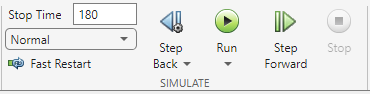
\includegraphics[width=0.6\textwidth]{taskBar.png}
}
\figcaption{Simulink TaskBar.}
\label{taskbar}
}%vbox
\end{center}

\noindent Všetko, čo potrebujete vedieť o možnostiach panelu zobrazeného na obrázku \ref{taskbar}, sú dve základné funkcie:  

\noindent Tlačidlo \uv{Run}, ktoré spustí simuláciu, a pole \uv{Stop Time}, ktoré určuje čas trvania experimentu.  


% section 2 -------------------------------------------------------------

\section{Opis blokovej schémy}

\noindent V tejto sekcii sa podrobnejšie pozrieme na samotnú blokovú schému, ktorá je znázornená na \ref{fig_blok_schema}. Ako je možné vidieť, schéma neobsahuje veľké množstvo prvkov a jej pochopenie by nemalo predstavovať problém.

\begin{center}
\vbox{%
\makebox[\textwidth][c]{%
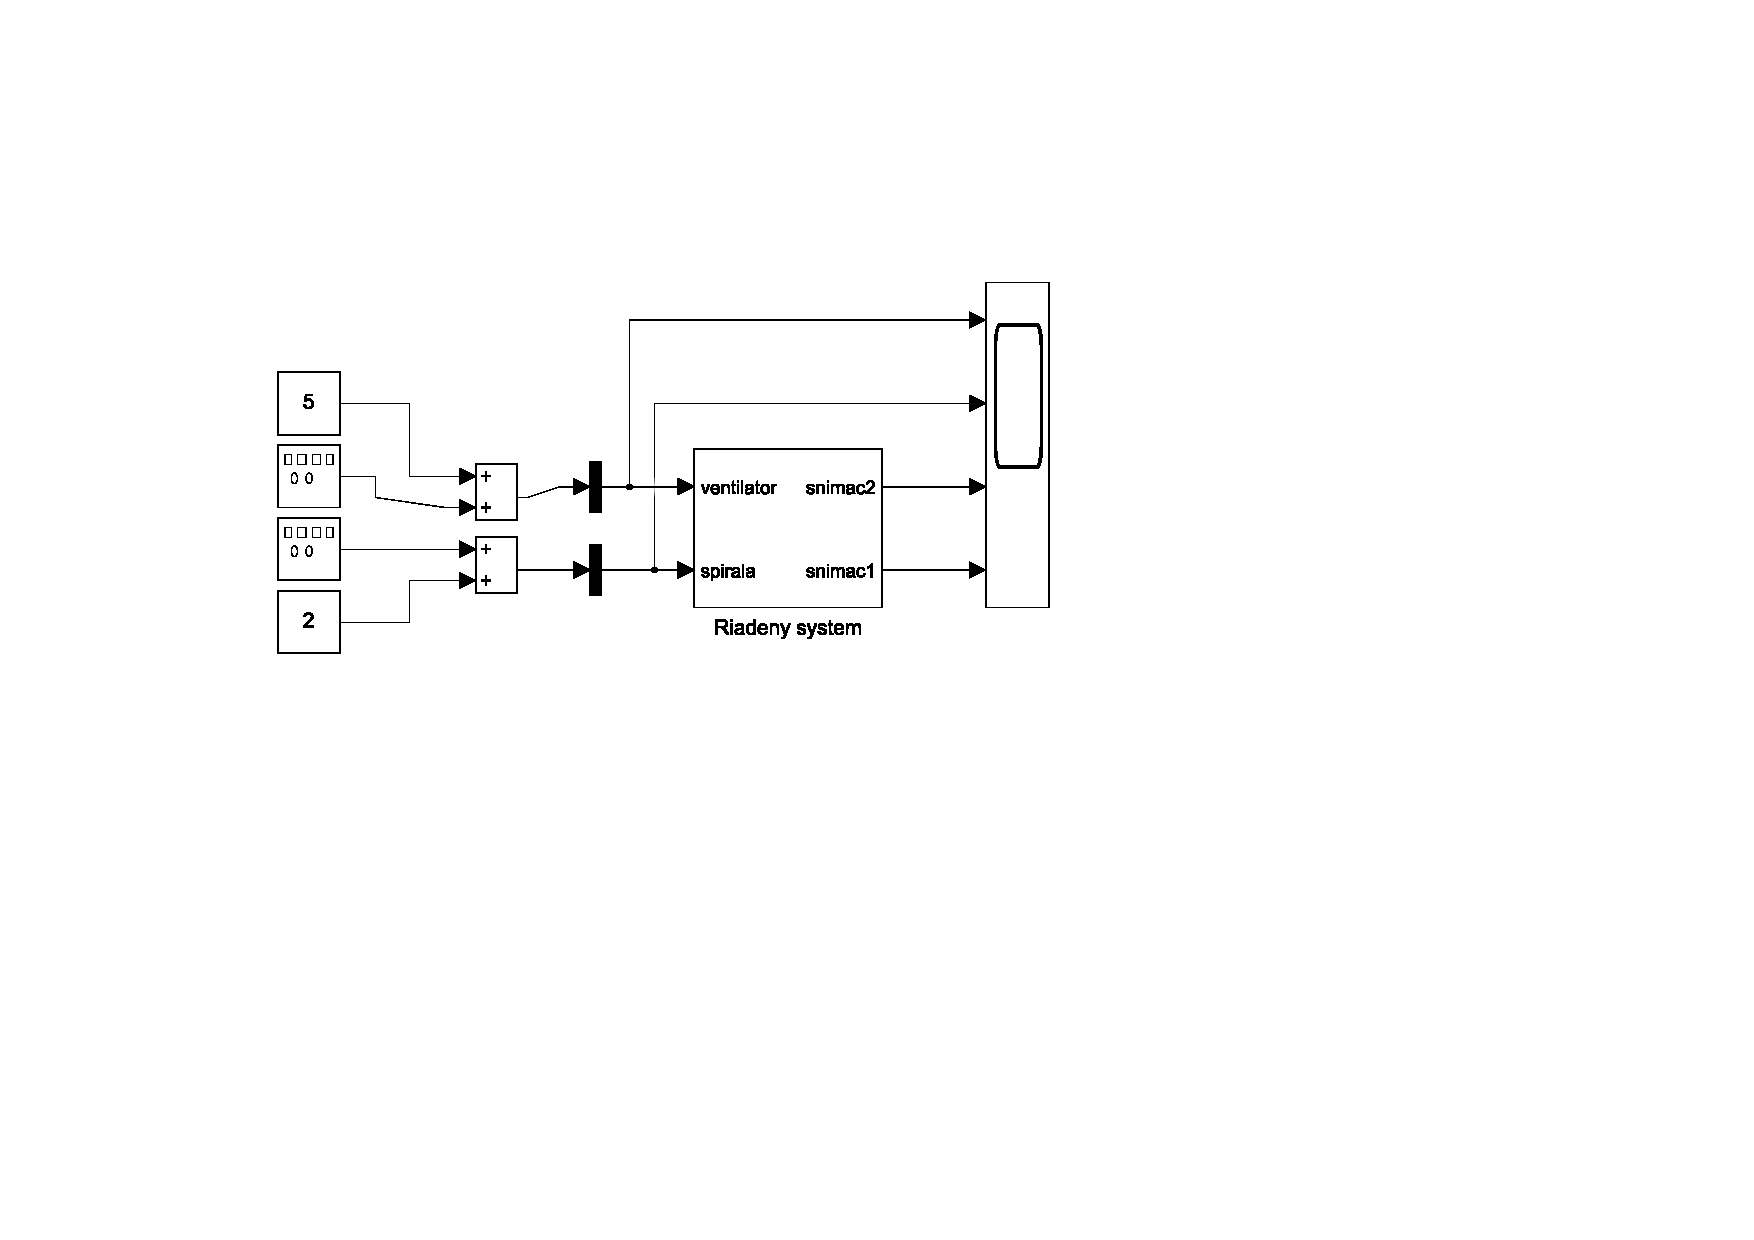
\includegraphics[width=1.1\textwidth, trim=100 250 300 130, clip]{TS05_basic_example.pdf}
}
\figcaption{Bloková schéma pre spustenie modelu TS05.}
\label{fig_blok_schema}
}%vbox
\end{center}

\noindent Prvým krokom sú samotné vstupy systému. Ide o dva generátory signálov. Jeden z nich produkuje sínusový signál s relatívne vysokou frekvenciou, ktorý slúži ako vstup pre ventilátor. Za týmto generátorom nasleduje blok so znamienkom „5“, čo predstavuje \uv{offset}. Offset znamená posun signálu smerom nahor alebo nadol o konštantnú hodnotu. Generátor signálu totiž v základnom nastavení nedisponuje parametrom offsetu a vytvára sínusový priebeh začínajúci od nuly s nastavenou amplitúdou a frekvenciou. Tieto parametre je možné meniť dvojitým kliknutím na blok a otvorením konfiguračného menu.  

\noindent Druhý vstup, určený pre špirálu, je konštrukčne podobný, avšak s iným offsetom (v tomto prípade 2) a iným tvarom aj frekvenciou signálu. Ide o štvorcový signál – teda skokovú zmenu. Prednastavené je, že skok nastane každých 60 sekúnd, čo zodpovedá frekvencii 1/120 Hz. V praxi to znamená, že jeden vstup sa neustále mení vplyvom sínusového priebehu, zatiaľ čo druhý sa mení skokovo raz za minútu, aby bolo možné sledovať odozvu systému na skokovú zmenu.  

\noindent Upozornenie: nie všetky schémy určené pre demo príklad obsahujú rovnaké parametre offsetu a signálu. Líšiť sa môže iba hodnota offsetu a amplitúdy, zatiaľ čo tvar aj frekvencia signálu zostávajú pre všetky modely rovnaké.

\noindent Ďalším kľúčovým prvkom je blok \uv{Riadeny system}. V kontexte tohto predmetu môže byť chápaný ako \uv{čierna skrinka}. V skutočnosti ide o blok, ktorý zabezpečuje prepojenie medzi prostredím Simulink a reálnou hardvérovou sústavou. Digitálny signál zo Simulinku je cez špeciálnu kartu v počítači prevedený na analógový signál (0–10 V), ktorý je následne privádzaný do reálneho modelu. Z modelu súčasne prichádzajú späť analógové signály (tiež 0–10 V), ktoré karta spracuje a odošle späť do prostredia MATLAB/Simulink na ďalšie spracovanie a vizualizáciu.  

\noindent Z bloku \uv{Riadeny system} vystupujú dve šípky, ktoré reprezentujú výstupy systému – konkrétne hodnoty ohrievania z blízkeho a vzdialeného senzora. Upozornenie: vždy si všimnite označenie vstupov a výstupov na bloku, pretože ich usporiadanie sa môže líšiť v závislosti od konkrétnej verzie schémy.  

\noindent Posledným prvkom je blok \uv{Scope}, ktorý umožňuje sledovať vstupy a výstupy systému v reálnom čase. Princíp je jednoduchý – signál pripojený k prvému portu sa zobrazí v prvom okne bloku Scope a tak ďalej. Aby bolo možné priebehy sledovať, je potrebné otvoriť blok Scope ešte pred spustením experimentu. Ak by ste ho otvorili počas behu experimentu, môže to viesť k chybe a pádu simulácie.  

\noindent Odporúčanie: pri prvom pokuse je vhodné spustiť experiment s otvoreným blokom Scope, aby ste mohli svoje výsledky porovnať s ukážkovými priebehmi uvedenými v nasledujúcej sekcii.  

\noindent Nebojte sa otvárať bloky, skúmať názvy ich parametrov a meniť ich nastavenia. Iba tak získate potrebné skúsenosti. Hardvéru prakticky nemôžete uškodiť, najhoršie, čo sa môže stať, je, že stratíte prehľad v schéme. V takom prípade si jednoducho stiahnite novú verziu z GitHubu.  

\begin{quote}
„Aby sme sa vyhli chybám, musíme získavať skúsenosti; a aby sme získali skúsenosti, musíme robiť chyby.“  
— Laurence J. Peter
\end{quote}

% section 3 -------------------------------------------------------------

\section{Výsledky demo príkladu}

\noindent V tejto sekcii sú bez detailných rozborov a hodnotenia prezentované výsledky spustenia demo príkladu \uv{TS05\_basic\_example.slx}. Treba zdôrazniť, že niektoré parametre vstupov sa v iných schémach môžu líšiť (konkrétne hodnoty offsetu a amplitúdy). Jediné, čo by malo zostať rovnaké, je približný tvar priebehov. Interpretácia a hodnotenie výsledkov je už vašou úlohou.  

\begin{center}
\vbox{%
\makebox[\textwidth][c]{%
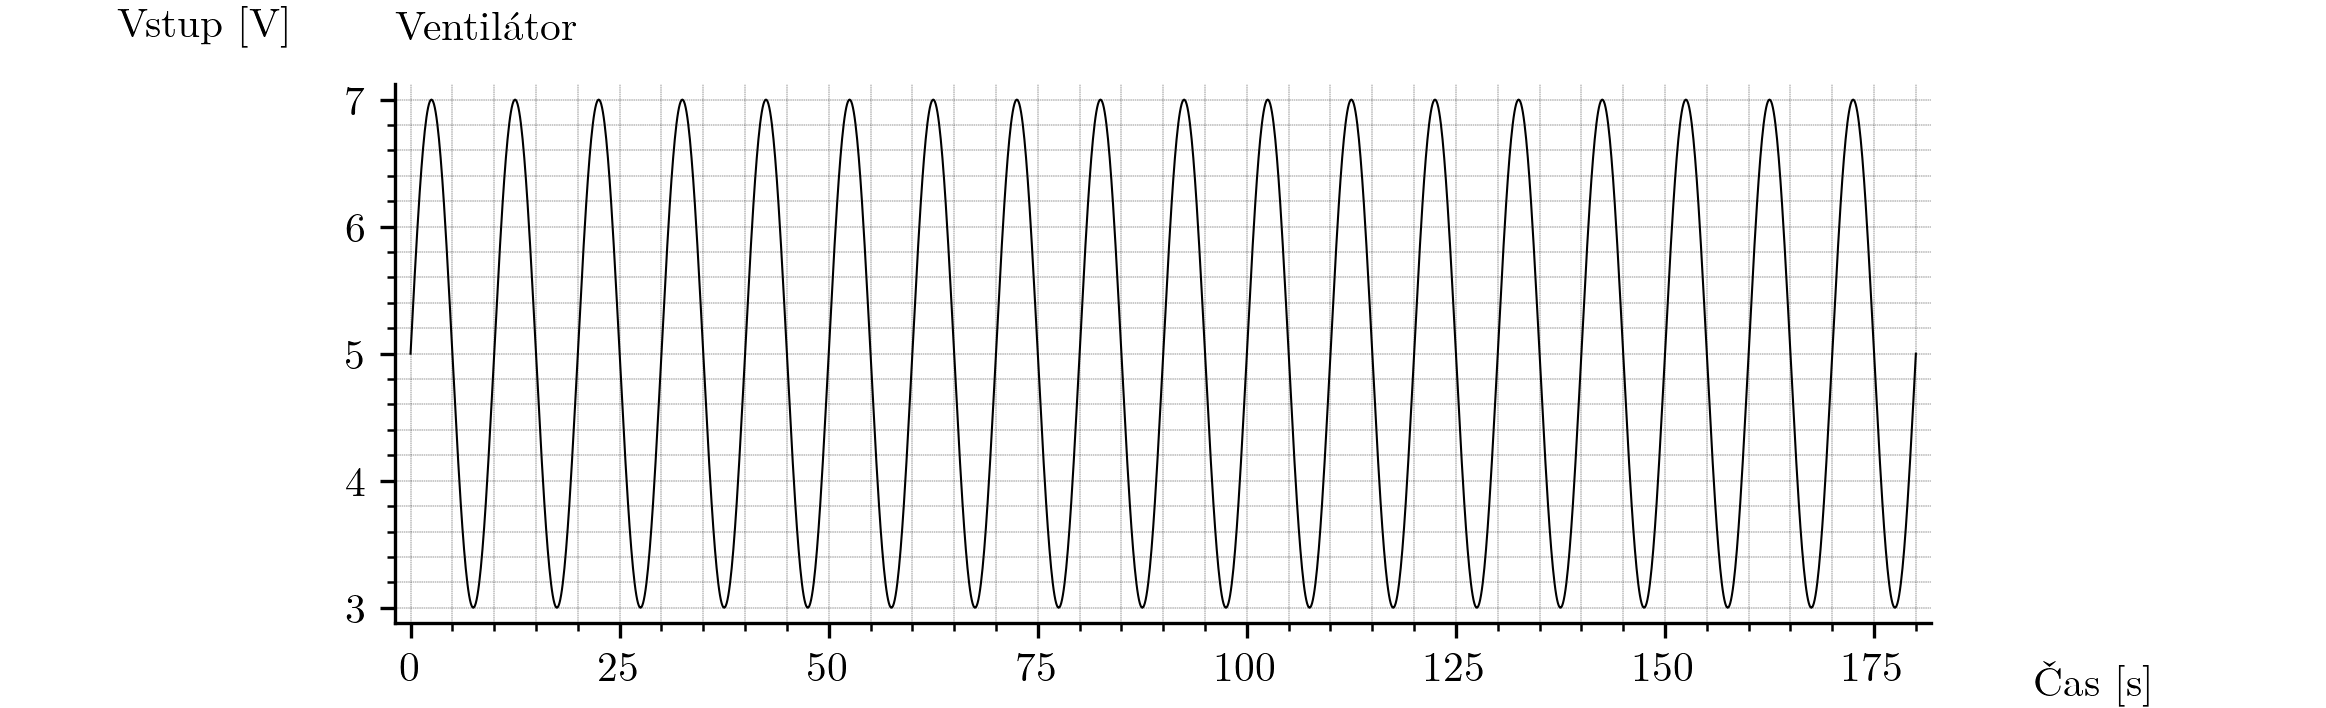
\includegraphics[width=1.5\textwidth]{ventilator_input.png}
}
\captionof{figure}{Vstupný signál – ventilátor.}
\label{fig_demo_vent}
}%vbox
\end{center}

\begin{center}
\vbox{%
\makebox[\textwidth][c]{%
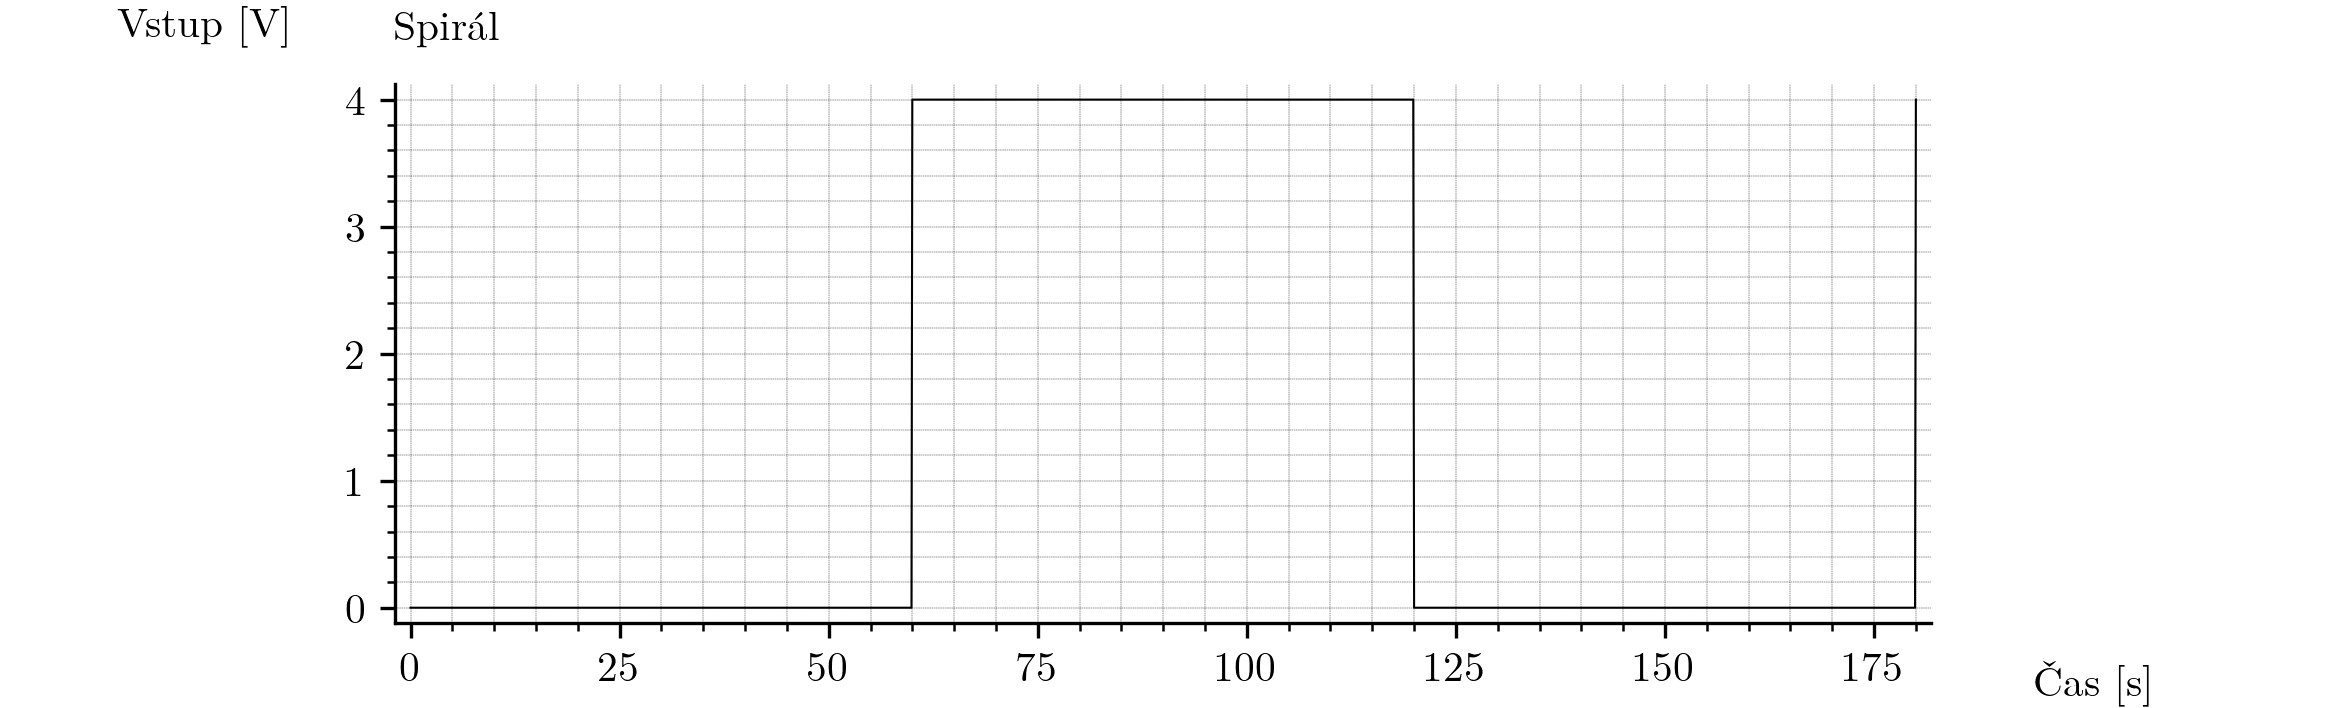
\includegraphics[width=1.5\textwidth]{spiral_input.png}
}
\captionof{figure}{Vstupný signál – špirála.}
\label{fig_demo_spiral}
}%vbox
\end{center}

\begin{center}
\vbox{%
\makebox[\textwidth][c]{%
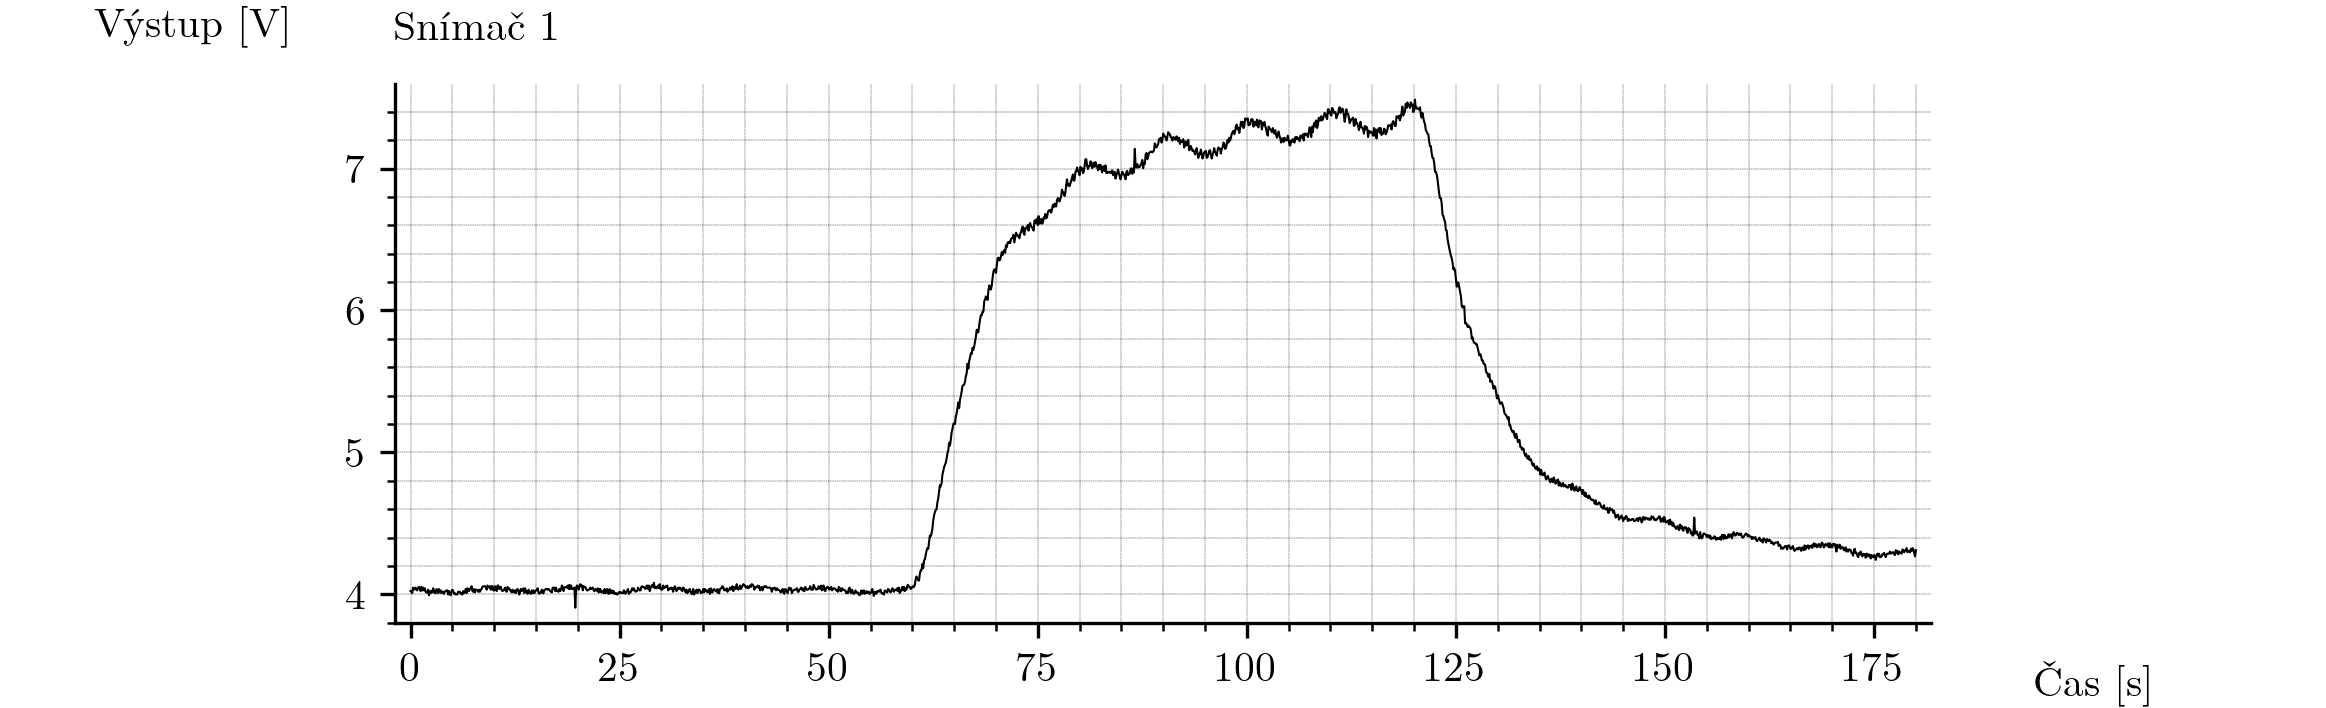
\includegraphics[width=1.5\textwidth]{snimac1_output.png}
}
\captionof{figure}{Výstupný signál – snímač 1.}
\label{fig_demo_sensor1}
}%vbox
\end{center}

\begin{center}
\vbox{%
\makebox[\textwidth][c]{%
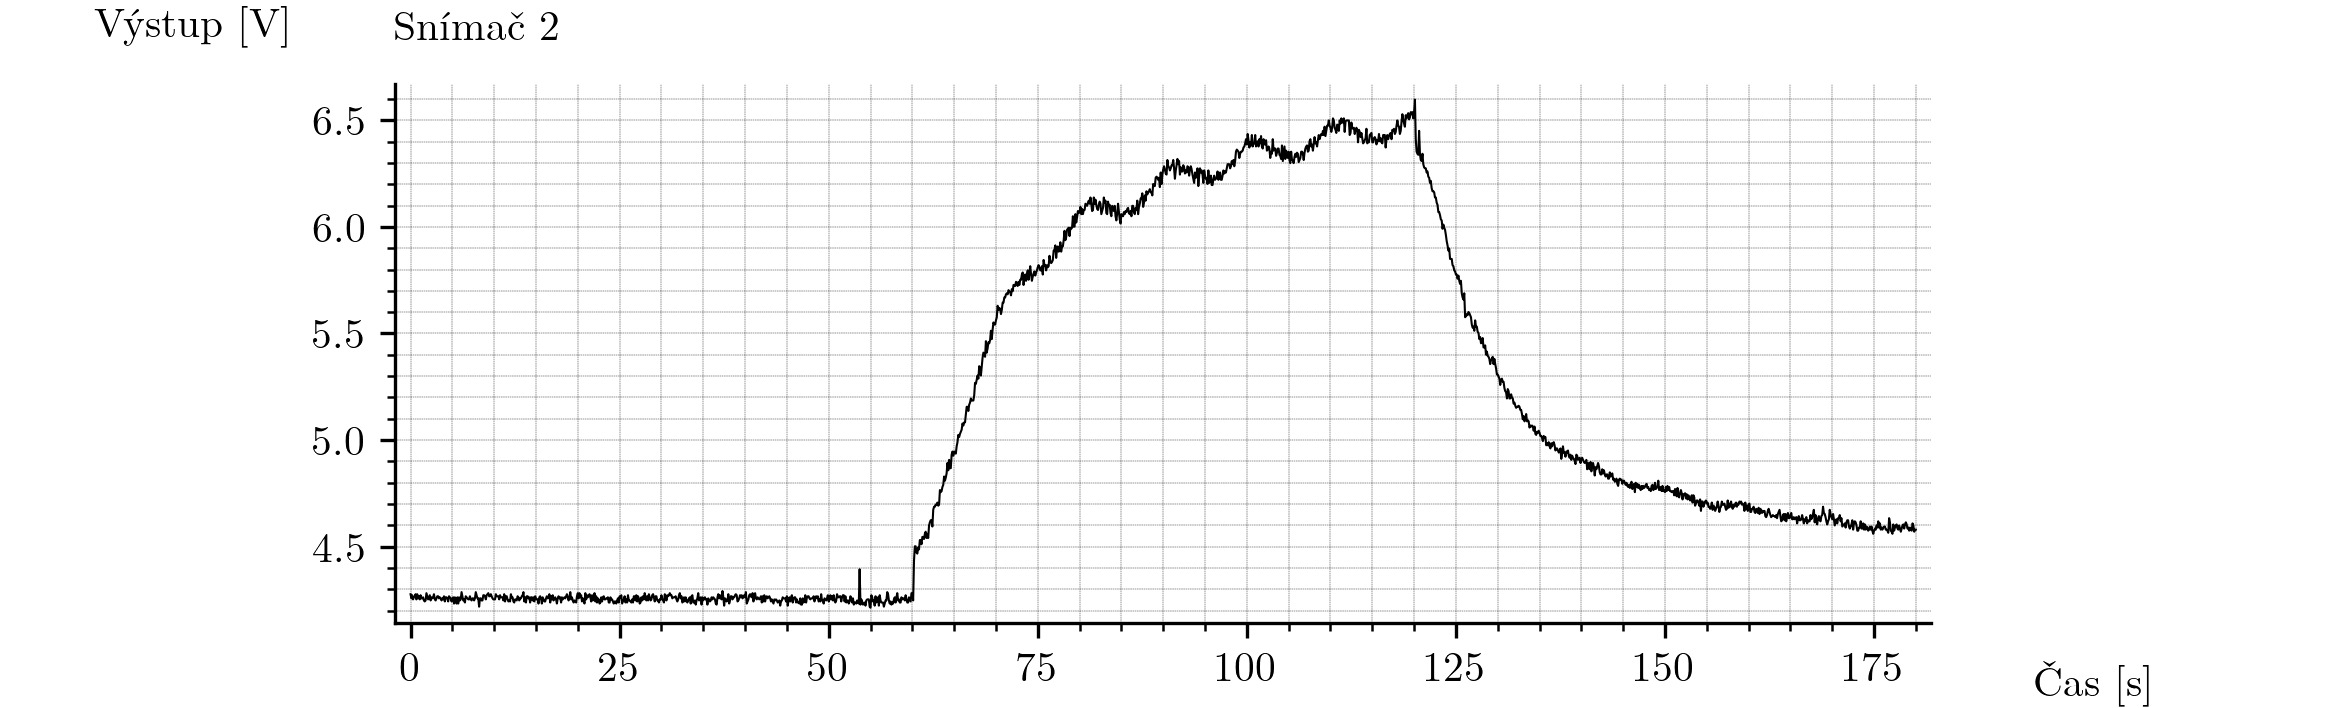
\includegraphics[width=1.5\textwidth]{snimac2_output.png}
}
\captionof{figure}{Výstupný signál – snímač 2.}
\label{fig_demo_sensor2}
}%vbox
\end{center}


%-----------------------------------------------------------------------------

\end{document}